\documentclass[tikz,border=10pt]{standalone}
\usepackage{amsmath,amssymb}
\usetikzlibrary{arrows.meta,positioning,fit,backgrounds}

% Fonts
\usepackage[T1]{fontenc}
\usepackage[utf8]{inputenc}
\usepackage{newpxtext,newpxmath}
\usepackage{sectsty}

\newcommand{\F}{\mathbb F}
\newcommand{\ideal}[1]{\langle #1\rangle}

\begin{document}
	
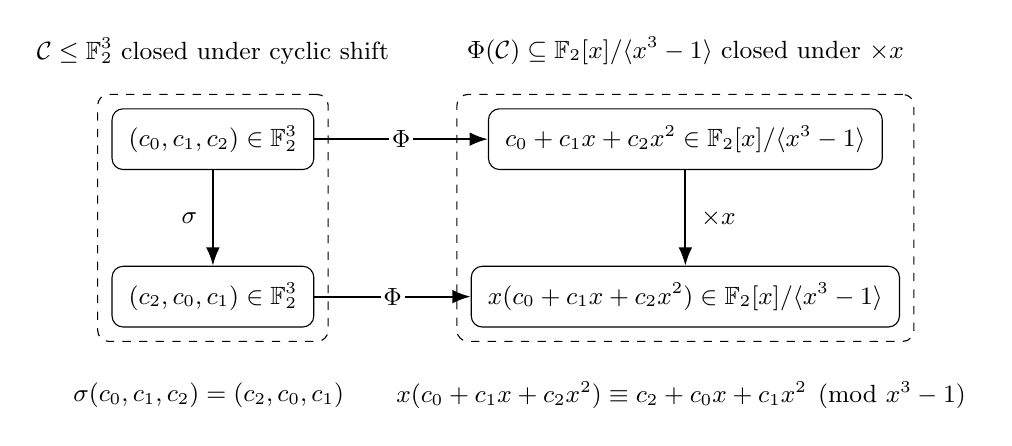
\begin{tikzpicture}[
	>=Latex,
	node distance=2.3cm and 3.8cm,
	every node/.style={font=\small},
	box/.style={draw, rounded corners, inner sep=6pt, align=center},
	subbox/.style={draw, rounded corners, dashed, inner sep=5pt, align=center},
	op/.style={midway, fill=white, inner sep=1pt}
	]
	
	%--- ambient spaces ---
	\node[box] (Vtop) at (0,2) {$(c_0,c_1,c_2)\in\F_2^3$};
	\node[box] (Vbot) at (0,0) {$(c_2,c_0,c_1)\in\F_2^3$};
	
	\node[box] (Rtop) at (6,2) {$c_0+c_1x+c_2x^2\in\F_2[x]/\ideal{x^3-1}$};
	\node[box] (Rbot) at (6,0) {$x(c_0+c_1x+c_2x^2)\in\F_2[x]/\ideal{x^3-1}$};
	
	%--- arrows of the commutative square ---
	\draw[->, thick] (Vtop) -- node[op] {$\Phi$} (Rtop);
	\draw[->, thick] (Vbot) -- node[op] {$\Phi$} (Rbot);
	
	\draw[->, thick] (Vtop) -- node[left=2pt] {$\sigma$} (Vbot);
	\draw[->, thick] (Rtop) -- node[right=2pt] {$\times x$} (Rbot);
	
	%--- highlighted code / ideal regions ---
	\node[subbox, fit={(Vtop) (Vbot)}, label={[yshift=.25cm]above:
		{$\mathcal C\le \F_2^3$ closed under cyclic shift}}] (Cbox) {};
	
	\node[subbox, fit={(Rtop) (Rbot)}, label={[yshift=.25cm]above:
		{$\Phi(\mathcal C)\subseteq \F_2[x]/\ideal{x^3-1}$ closed under $\times x$}}] (Ibox) {};
	
	%--- lower explanatory labels ---
	\node[align=center] at (0,-1.25)
	{
		\(\sigma(c_0,c_1,c_2)=(c_2,c_0,c_1)\)
%		\\[2pt]
%		cyclic shift
	};
	
	\node[align=center] at (6,-1.25)
	{
		\(x(c_0+c_1x+c_2x^2)\equiv c_2+c_0x+c_1x^2 \pmod{x^3-1}\)
%		\\[2pt]
%		multiplication by \(x\)
	};
	
%	%--- conclusion arrow ---
%	\draw[->, very thick] (3.1,-2.2) -- (5.9,-2.2);
%	\node[align=center] at (4.5,-2.75)
%	{
%		\(\mathcal C\) is \(\F_2\)-linear and stable under \(\sigma\)\\
%		\(\Longrightarrow\) \(\Phi(\mathcal C)\) is closed under addition and \(\times x\)\\
%		\(\Longrightarrow\) closed under multiplication by every polynomial\\
%		\(\Longrightarrow\) \(\Phi(\mathcal C)\) is an ideal
%	};
	
\end{tikzpicture}
	
\end{document}